%%%%%%%%%%%%%%%%%%%%%%%%%%%%%%%%%%%%%%%%%
% Beamer Presentation
% LaTeX Template
% Version 1.0 (10/11/12)
%
% This template has been downloaded from:
% http://www.LaTeXTemplates.com
%
% License:
% CC BY-NC-SA 3.0 (http://creativecommons.org/licenses/by-nc-sa/3.0/)
%
%%%%%%%%%%%%%%%%%%%%%%%%%%%%%%%%%%%%%%%%%

%----------------------------------------------------------------------------------------
%	PACKAGES AND THEMES
%----------------------------------------------------------------------------------------

\documentclass{beamer}

\mode<presentation> {

% The Beamer class comes with a number of default slide themes
% which change the colors and layouts of slides. Below this is a list
% of all the themes, uncomment each in turn to see what they look like.

%\usetheme{default}
%\usetheme{AnnArbor}
%\usetheme{Antibes}
%\usetheme{Bergen}
%\usetheme{Berkeley}
%\usetheme{Berlin}
%\usetheme{Boadilla}
%\usetheme{CambridgeUS}
%\usetheme{Copenhagen}
%\usetheme{Darmstadt}
%\usetheme{Dresden}
%\usetheme{Frankfurt}
%\usetheme{Goettingen}
%\usetheme{Hannover}
%\usetheme{Ilmenau}
%\usetheme{JuanLesPins}
%\usetheme{Luebeck}
\usetheme{Madrid}
%\usetheme{Malmoe}
%\usetheme{Marburg}
%\usetheme{Montpellier}
%\usetheme{PaloAlto}
%\usetheme{Pittsburgh}
%\usetheme{Rochester}
%\usetheme{Singapore}
%\usetheme{Szeged}
%\usetheme{Warsaw}

% As well as themes, the Beamer class has a number of color themes
% for any slide theme. Uncomment each of these in turn to see how it
% changes the colors of your current slide theme.

%\usecolortheme{albatross}
%\usecolortheme{beaver}
%\usecolortheme{beetle}
%\usecolortheme{crane}
%\usecolortheme{dolphin}
%\usecolortheme{dove}
%\usecolortheme{fly}
%\usecolortheme{lily}
%\usecolortheme{orchid}
%\usecolortheme{rose}
%\usecolortheme{seagull}
%\usecolortheme{seahorse}
%\usecolortheme{whale}
%\usecolortheme{wolverine}

%\setbeamertemplate{footline} % To remove the footer line in all slides uncomment this line
%\setbeamertemplate{footline}[page number] % To replace the footer line in all slides with a simple slide count uncomment this line

%\setbeamertemplate{navigation symbols}{} % To remove the navigation symbols from the bottom of all slides uncomment this line
}

\usepackage{graphicx} % Allows including images
\usepackage{booktabs} % Allows the use of \toprule, \midrule and \bottomrule in tables
\usepackage[brazilian]{babel}
\usepackage[utf8]{inputenc}
\usepackage{listings}
\usepackage{amsmath}
\usepackage{amsfonts}

\graphicspath{ {img/} }

%----------------------------------------------------------------------------------------
%	Macros para definir programa linear
%----------------------------------------------------------------------------------------
\makeatletter
\newcommand{\minproblem}{\@ifstar\minproblemstar\minproblemplain}
\newcommand{\minproblemplain}[3][]{
  \begin{align}
    \text{#1}\textbf{minimiza}\qquad & #2\\
    \textbf{subjeito a}\qquad & #3
  \end{align}
}
\newcommand{\minproblemstar}[3][]{
  \begin{align*}
    \text{#1}\textbf{minimiza}\qquad & #2\\
    \textbf{subjeito a}\qquad & #3
  \end{align*}
}
\newcommand{\maxproblem}{\@ifstar\maxproblemstar\maxproblemplain}
\newcommand{\maxproblemplain}[3][]{
  \begin{align}
    \text{#1}\textbf{maximiza}\qquad & #2\\
    \textbf{subjeito a}\qquad & #3
  \end{align}
}
\newcommand{\maxproblemstar}[3][]{
  \begin{align*}
    \text{#1}\textbf{maximiza}\qquad & #2\\
    \textbf{subjeito a}\qquad & #3
  \end{align*}
}
\makeatother

%----------------------------------------------------------------------------------------
%	TITLE PAGE
%----------------------------------------------------------------------------------------

\title[Simulated Annealing + Redes Virtuais]{Aplicação da Meta-heurística Simulated Annealing para solução do problema de Mapeamento de Redes Virtuais} % The short title appears at the bottom of every slide, the full title is only on the title page

\author[Fernando]{Fernando Bombardelli da Silva (218324)} % Your name
\institute[UFRGS] % Your institution as it will appear on the bottom of every slide, may be shorthand to save space
{
Universidade Federal do Rio Grande do Sul \\ % Your institution for the title page
Instituto de Informática \\
\medskip
\textit{fbdasilva@inf.ufrgs.br} % Your email address
}
\date{\today} % Date, can be changed to a custom date

\begin{document}

\begin{frame}
\titlepage % Print the title page as the first slide
\end{frame}

\begin{frame}
\frametitle{Visão Geral} % Table of contents slide, comment this block out to remove it
\tableofcontents % Throughout your presentation, if you choose to use \section{} and \subsection{} commands, these will automatically be printed on this slide as an overview of your presentation
\end{frame}

%----------------------------------------------------------------------------------------
%	PRESENTATION SLIDES
%----------------------------------------------------------------------------------------

%------------------------------------------------
\section{Introdução} % Sections can be created in order to organize your presentation into discrete blocks, all sections and subsections are automatically printed in the table of contents as an overview of the talk
%------------------------------------------------

%\subsection{Subsection Example} % A subsection can be created just before a set of slides with a common theme to further break down your presentation into chunks

\begin{frame}
\frametitle{Introdução | Caracterização do Problema}
\begin{itemize}
\item \textbf{Entrada:} Um grafo virtual e um grafo do substrato físico
\item \textbf{Problema de Localização:} Encontrar um mapeamento \emph{válido} dos vértices do grafo virtual para os vértices do grafo físico, assim como das arestas do virtual para caminhos no físico
\item \textbf{Problema de Otimização:} Minimizar a banda total utilizada pelo mapeamento
\end{itemize}
\end{frame}

\begin{frame}
\frametitle{Introdução | Formulação Matemática}
\begin{figure}
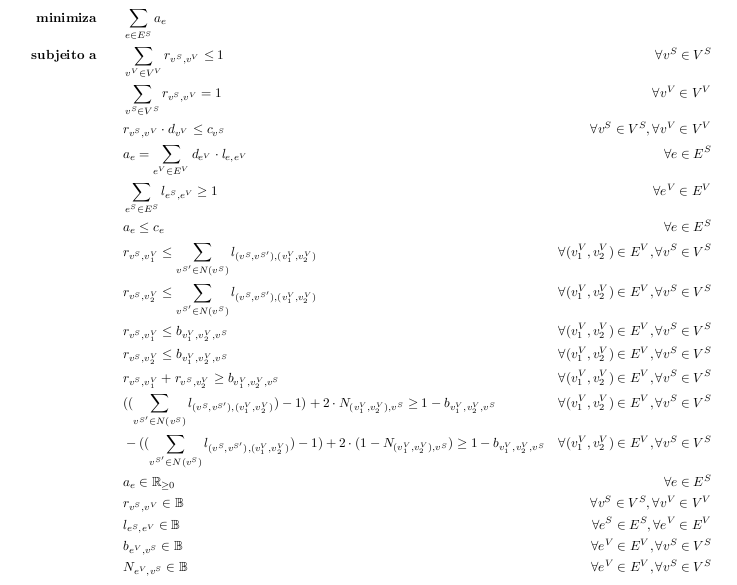
\includegraphics[scale=0.35]{prog_linear}
\end{figure}
\end{frame}

%------------------------------------------------
\section{Descrição da Solução}
%------------------------------------------------

\begin{frame}
\frametitle{Descrição da Solução | Representação da Solução}
\begin{itemize}
\item Par ordenado \textbf{\emph{(f(v), g(e))}}, onde \textbf{\emph{\(v \in V^{V}\)}} e \textbf{\emph{\(e \in E^{V}\)}}. Ou seja, o primeiro componente representa uma função, cujo domínio é o conjunto de vértices virtuais e o contra-domínio é o conjunto de vértices físicos; e o segundo componente representa uma função, cujo domínio é o conjunto de arestas virtuais e o contra-domínio é o conjunto de todas as tuplas que representem caminhos entre as arestas físicas.
\item Função Objetivo
\end{itemize}

\begin{displaymath}
\sum_{e \in E^{V}} d_{e} \cdot NroVertices(g(e))
\end{displaymath}
\end{frame}

\begin{frame}
\frametitle{Descrição da Solução | Solução Inicial}
\begin{itemize}
\item A ideia do algoritmo implementado é a seguinte:
	\begin{itemize}
	\item Seleciona uma aresta virtual e mapeia seus vértices adjacentes
	\item Escolhe um caminho possível entre os dois vértices físicos
	\item Volta ao passo um (de forma recursiva), porém com uma aresta virtual adjacente à recém alocada (se possível)
	\end{itemize}
\item \textit{"Percorre o grafo virtual aresta a aresta tentando mapear vértices e caminhos físicos."}
\item Alternativa: Análise topológica dos grafos
\end{itemize}
\end{frame}

\begin{frame}
\frametitle{Descrição da Solução | Vizinhança}
\begin{itemize}
\item Nessa implementação utilizou-se um algoritmo que segue os seguintes passos:
\begin{enumerate}
\item Seleciona randomicamente um vértice virtual;
\item Remove-o da solução, assim como os caminho referentes aos vértices adjacentes a ele;
\item Randomiza um novo vértice físico capaz de ser alocado para este vértice virtual;
\item Para cada vértice adjacente ao virtual, tenta estabelecer um caminho ao novo vértice físico, em caso de não possibilidade, voltar ao passo 1 e repetir os passos até que alcance um limite de iterações ou uma solução factível seja encontrada.
\end{enumerate}
\end{itemize}
\end{frame}

\begin{frame}
\frametitle{Descrição da Solução | Temperatura Inicial e Critério de Parada}
\begin{itemize}
\item \textbf{Temperatura Inicial:} Versão reduzida do algoritmo. Objetiva achar a maior variação de energia em relação à solução inicial.
\begin{displaymath}
\frac{-variacaoMaxima}{\ln p}
\end{displaymath}
\item \textbf{Critério de Parada:} Ficaram estabelecidos dois critérios de parada, que são informados por parâmetro:
	\begin{enumerate}
	\item Ocorrer uma iteração mais externa com um número de melhorias na solução seja menor do que o limiar;
	\item o número de iterações externas atingir um máximo estipulado.
	\end{enumerate}
\item O algoritmo para assim que alguma dessas condições for verdadeira.
\end{itemize}
\end{frame}

%------------------------------------------------
\section{Resultados}
%------------------------------------------------

\begin{frame}
\frametitle{Implmentação dos algoritmos}
\begin{itemize}
\item \textbf{\emph{Solver} GNU GLPK:} Execução por um longo período sem produção de resultados finais
\item \textbf{\emph{Simulated Annealing} em Python 3}
\end{itemize}
\begin{table}[H]
\centering
\begin{tabular}{|l | r |}
	\hline
	\textbf{Parâmetro} & \textbf{Valor} \\ \hline
	Iterações externas		& 1000	\\ \hline
	Iterações internas		& 300	\\ \hline
	Mínimo de iterações com sucesso	& 10 	\\ \hline
	Coeficiente de resfriamento		& 0.99	\\ \hline
\end{tabular}
\caption{Parâmetros do Algoritmo}
\label{tab:Parametros}
\end{table}
\end{frame}

\begin{frame}
\frametitle{Resultados}

\footnotesize{
\begin{table}[H]
\centering
\begin{tabular}{|l | r | r | r | r | r|}
	\hline
	\textbf{Inst.} & \textbf{Sol.Inicial} & \textbf{Sol.Final} & \textbf{Desvio à Ini.} & \textbf{Desvio à Ótima} & \textbf{Minutos} \\ \hline
	sub1	& 1236	& 874	& 29,29\%	& 228,57\%	& 25	\\ \hline
	sub2	& 2232	& 1512	& 32,26\%	& 440,00\%	& 50	\\ \hline
	sub3	& 3414	& 2226	& 34,8\%	& 428,74\%	& 39	\\ \hline
	sub4	& 3602	& 3602 	& 0,0\%		& 456,72\%	& 90	\\ \hline
	sub5	& 2728	& 2178	& 20,16\%	& 379,74\%	& 44	\\ \hline
\end{tabular}
\caption{Resultados das Computações}
\label{tab:Resultado}
\end{table}
As instâncias \emph{ts1}, \emph{ts2}, \emph{ts3}, \emph{ts4} e \emph{ts5} não puderam ser otimizadas, pois a busca por uma solução inicial levou muito tempo e não foi possível produzir resultado.

Principal Limitante para a convergência: Algoritmo de vizinhança.
}
\end{frame}


%------------------------------------------------
\section{Conclusão}
%------------------------------------------------

\begin{frame}
\frametitle{Conclusão}
\begin{itemize}
\item Mapeamento de redes virtuais é complexo até mesmo para localização de solução inicial
\item Importância do algoritmo de vizinhança para uma boa convergência do método
\item \emph{Solvers} genéricos não são viáveis na prática
\item Decisões na fase de projeto do algoritmo são cruciais para o resultado com a meta-heurística
\end{itemize}
\end{frame}

%------------------------------------------------

\begin{frame}
\frametitle{Referências}
\footnotesize{
\begin{thebibliography}{1}
\bibitem{Melo}
	Melo, M.; Carapinha, J.; Sargento, S.; Torres, L.; Tran-Phuong, N.; Killat Killat, U.; Timm-Giel, A.;
	\emph{Virtual Network Mapping - An Optimization Problem}.
	Conference on Mobile Networks and Management (MONAMI).
	Aveiro, Portugal, 2011.
\bibitem{}
	Xiaoling Li; Changguo Guo; Huaimin Wang; Zhendong Li; Zhiwen Yang;
	\emph{A constraint optimization based virtual network mapping method}.
	International Conference on Graphic and Image Processing (ICGIP).
	Singapore, Singapore, 2012.
\bibitem{}
	Peterson, Carsten; Söderberg, Bo;
	\emph{A New Method For Mapping Optimization Problems Onto Neural Networks}.
	International Journal of Neural Systems.
	1989.
\bibitem{AMPL}
	Fourer, Robert; Gay, David M.; Kernighan, Brian W.;
	\emph{AMPL: A Modeling Language for Mathematical Programming}.
	2$^{nd}$ Ed.
	Disponível em: $<$http://ampl.com/resources/the-ampl-book/$>$.
	2003.
\bibitem{}
	Paragon Decision Technology.
	\emph{AIMMS Modeling Guide - Linear Programming Tricks}.
	Disponível em: $<$http://www.aimms.com/aimms/download/manuals/aimms3om\_linearprogrammingtricks.pdf$>$.
	1993.
\end{thebibliography}
}
\end{frame}

\begin{frame}
\frametitle{Referências}
\footnotesize{
\begin{thebibliography}{6}
\bibitem{ABSOLUTE}
	Lp Solve Reference Guide.
	\emph{Absolute Values}.
	Disponível em: $<$http://lpsolve.sourceforge.net/5.1/absolute.htm$>$.
	Acesso em: Junho de 2014.
\bibitem{GLPK}
	Free Software Foudation.
	\emph{GLPK - GNU Project}.
	Disponível em: $<$http://www.gnu.org/software/glpk/$>$.
	Acesso em: Maio de 2014.
\bibitem{PYTHON}
	Python Software Foundation.
	\emph{Python 3.4.1 documentation}.
	Disponível em: $<$https://docs.python.org/3/$>$.
	Acesso em: Junho de 2014.
\bibitem{}
	Wikipedia.
	\emph{Monte Carlo method}.
	Disponível em: $<$http://en.wikipedia.org/wiki/Monte\_Carlo\_method$>$.
	Acesso em: Junho de 2014.
\end{thebibliography}
}
\end{frame}
%------------------------------------------------

\begin{frame}
\Huge{\centerline{Fim}}
\end{frame}

%----------------------------------------------------------------------------------------

\end{document}